\documentclass[tikz,border=3.14mm]{standalone}
\usepackage{tikz}
\begin{document}
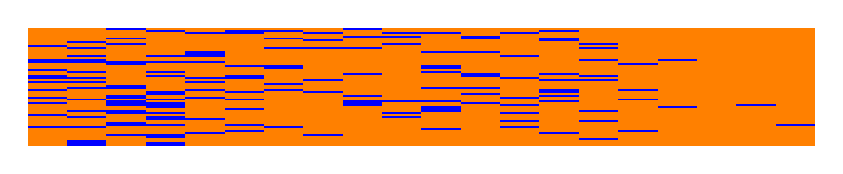
\begin{tikzpicture}
\foreach \i in {0,...,59}{
    \foreach \j in {0,...,19}{
        \pgfmathsetmacro\prob{(\j)/20 * 0.5 + 0.5} % Compute the probability of being orange
        \pgfmathparse{rand<\prob?1:0} % Generate a random number and compare with the probability
        \ifnum\pgfmathresult=0 % If the generated number is less than the probability, the rectangle is orange
            \fill[blue] (\j*0.5,\i*0.025) rectangle ++(0.5,0.025);
        \else % Else, the rectangle is blue
            \fill[orange] (\j*0.5,\i*0.025) rectangle ++(0.5,0.025);
        \fi
    }
}
\end{tikzpicture}
\end{document}
